A \textit{treap}, also known as \textit{Cartesian tree}, is a data structure that stores a set of keys in a binary search tree.

Each node of this tree is characterized by a pair $(x, y)$. 

The $x$ values of the nodes are the stored keys. They obey ``the binary search tree rule'': all $x$ values in the left subtree of the node are smaller than its $x$ value, and all $x$ values in the right subtree of the node are larger than its $x$ value.

The $y$ values of the nodes obey ``the heap rule'': $y$ value of a node is less than or equal to the $y$ value of its parent.
 
The $y$ value for each created node is usually selected randomly according to some distribution. This results in nice average time complexity of many operations.

Since this data structure unites some properties of a binary search tree and a heap, its name is a ``portmanteau'' term made of two words: TRee + hEAP = TREAP.

\begin{center}
\begin{tabular}{c@{\hspace{5em}}c}
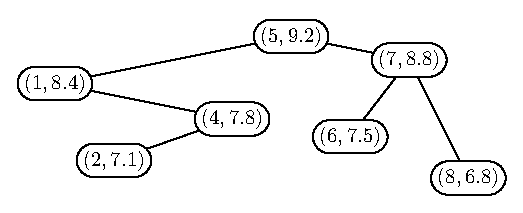
\includegraphics{treap-1.ps} & \includegraphics{treap-2.ps}\\
A treap with 7 nodes; its height is 4 & A treap for the sample test below\\
\end{tabular}
\end{center}

Benjamin decided that nondeterminism in $y$ value selection procedure is bad, as it makes execution time differ from one run to another. He decided to calculate $y$ for each node deterministically based on its $x$. He selected the rule $y = \sin(x)$. He is especially glad that distinct integer $x$'s will always have distinct $y$'s.

Barbara understands that while the nondeterministic treap shows its worst performance when provided ``bad'' random sequence, the deterministic treap shows its worst performance when provided ``bad'' set of keys. She wants to explain it to Benjamin by showing him $n$ integer keys, which, being stored in his data structure, will form a treap of height $n$~--- the ``most unbalanced'' possible situation.

Help Barbara by providing $n$ such keys. All these keys should fit into the 32-bit signed integer type.